\documentclass[a4paper]{jpconf}
\usepackage{graphicx}
\usepackage{wrapfig}

\begin{document}
\title{Systematic profiling to monitor and specify the software refactoring process of the LHCb experiment}

\author{Ben Couturier}
\address{CERN, CH-1211 Geneva 23, Switzerland}
\ead{ben.couturier@cern.ch}

\author{Emmanouil Kiagias}
\address{CERN, CH-1211 Geneva 23, Switzerland}
\ead{emmanouil.kiagias@cern.ch}

\author{Stefan B. Lohn}
\address{CERN, CH-1211 Geneva 23, Switzerland}
\ead{stefan.lohn@cern.ch}

\begin{abstract}
The LHCb collaboration develops and maintains large software frameworks for the LHCb and other experiments based on Gaudi. In the upcoming years a big refactoring effort is planned to introduce features like vectorization, parallelization, to minimize hotspots and to reduce the impact of bottlenecks. It is crucial to guide the refactoring with a profiling system that gives hints to parts for possible and necessary source-code reengineering and which kind of optimization could lead to final success. From detailed profiling few results are selected, summarized and available to be visualized by a web analysis frontend.
%More detailed information can be accessed via files to download or in case access from AFS, the internal network file system.
\newline
Software optimization is a sophisticated process where all parts, compiler, operating system, libraries and chosen hardware play a role in. Intended improvements can have different effects on different platforms. To obtain precise information of the general performance, to make profiles comparable, reproducible and to verify the progress of performance in the framework, it is important to produce profiles more systematically in terms of regular profiling based on representative use cases and to perform regression tests. Once a general execution, monitoring and analysis platform is available, software metrics can be derived from the collected profiling results to trace changes in performance back and to create summary reports on a regular basis with an alert system if modifications led to significant performance degradations.
\end{abstract}

\newpage

\section{Introduction}
\label{sec:introduction}

To assure that software performance of a large-scale framework keeps its preestimated performance boundaries, regular and detailed profiling is indispensable. Since software is not going to speed up anymore with each new generation of cpu's, profiling tools to trace back hotspots and to discover interesting regions to optimize the cpu's exploitation are becoming more and more important. But profiling was not an integral part of the software development procedure of the LHCb experiment for the first period of the LHC run till 2013. line-number-modeProfiling remained an unsystematic task which each developer or collaborating development group conducted on its own. Profiles were thus only of temporal value, incomparable and often unreproducible. This paper is not going to evaluate the benefits and drawbacks of different tools, but wants to enable the collaboration to systematize profiling and to make progress comparable and more visible for the upcoming refactoing face to make the source-code ready for the second big LHCb run.
\newline
Important objectives to develop a framework for regular systematic profiling are, to be aware of comparability, reproducibility and automation of performance validation. ...
\newline
This paper is organized ...

\section{LHCb computing}
\label{sec:lhcb_computing}



\subsection{LHCb software}
\label{sec:lhcb_software}

The software frameworks used in the LHCb experiment are based on Gaudi \cite{gaudi}. Gaudi is a framework using generic and object-oriented features of C++ for processing intensive tasks and python for configuring and structuring modules, which we call algorithms. It executes consecutive an abstract series of these algorithms to process data objects from the transient store on request. Gaudi is providing core services and tools for applications to hide complexity and make future development and changes more transparent for users. It is a large-scale framework and is used by ATLAS, Glast, Harp and other experiments.
\newline
Applications build on top of Gaudi are Brunel, Gauss, DaVinci, Moore, Boole and others. Moore is the implementation of the high-level trigger to decide weather event data will be stored or not. Brunel is responsible for the offline reconstruction, Gauss is simulating the particle transport and interaction through detector modules, and Boole performs the digitization.

\subsection{Integrated Profiling}
\label{sec:integrated_profiling}

In HEP computing it is a common method to measure performance via throughput (events per time unit). Thus the performance analysis is focused on the time linear and not the time constant part of processing like initialization. To achieve this, instrumentation is an important advantage for profiling source-code in a large scale frameworks like those from the LHCb experiment. Multiple profilers and measurements have been implemented in the Gaudi framework using the Auditor-Service. Timing information from the operating system's process information are collected using the TimingAuditor and printing a summary of time spend in the applications algorithms. Likewise memory information can be collected using the MemoryAuditor as soon as changes in memory consumption are observed. Recently the API of Intel's VTune Amplifier was used by Mazurov and Couturier \cite{intel_auditor} to implement an IntelAuditor to be used for profiling the event loop with higher precision. Another strategy is to collect information from the PMU of a modern CPU architecture to collect information about hardware related issues, such as cach-misses, branch-misprediction and stall cycles as done by Kruse and Kruzelecki \cite{monitoring} for the Gaudi framework.

\subsection{Computing environment}
\label{sec:computing_environment}

The LHCb computing environment persists in particular out of the WLCG and (what ever is in the pit). Around (N) CPU's are processing data collected by the different detector subsystems. M GB of recorded data per second have to be processed by N computing nodes the high-level-trigger (HLT) to decide if they should be stored.

\begin{figure}{t}
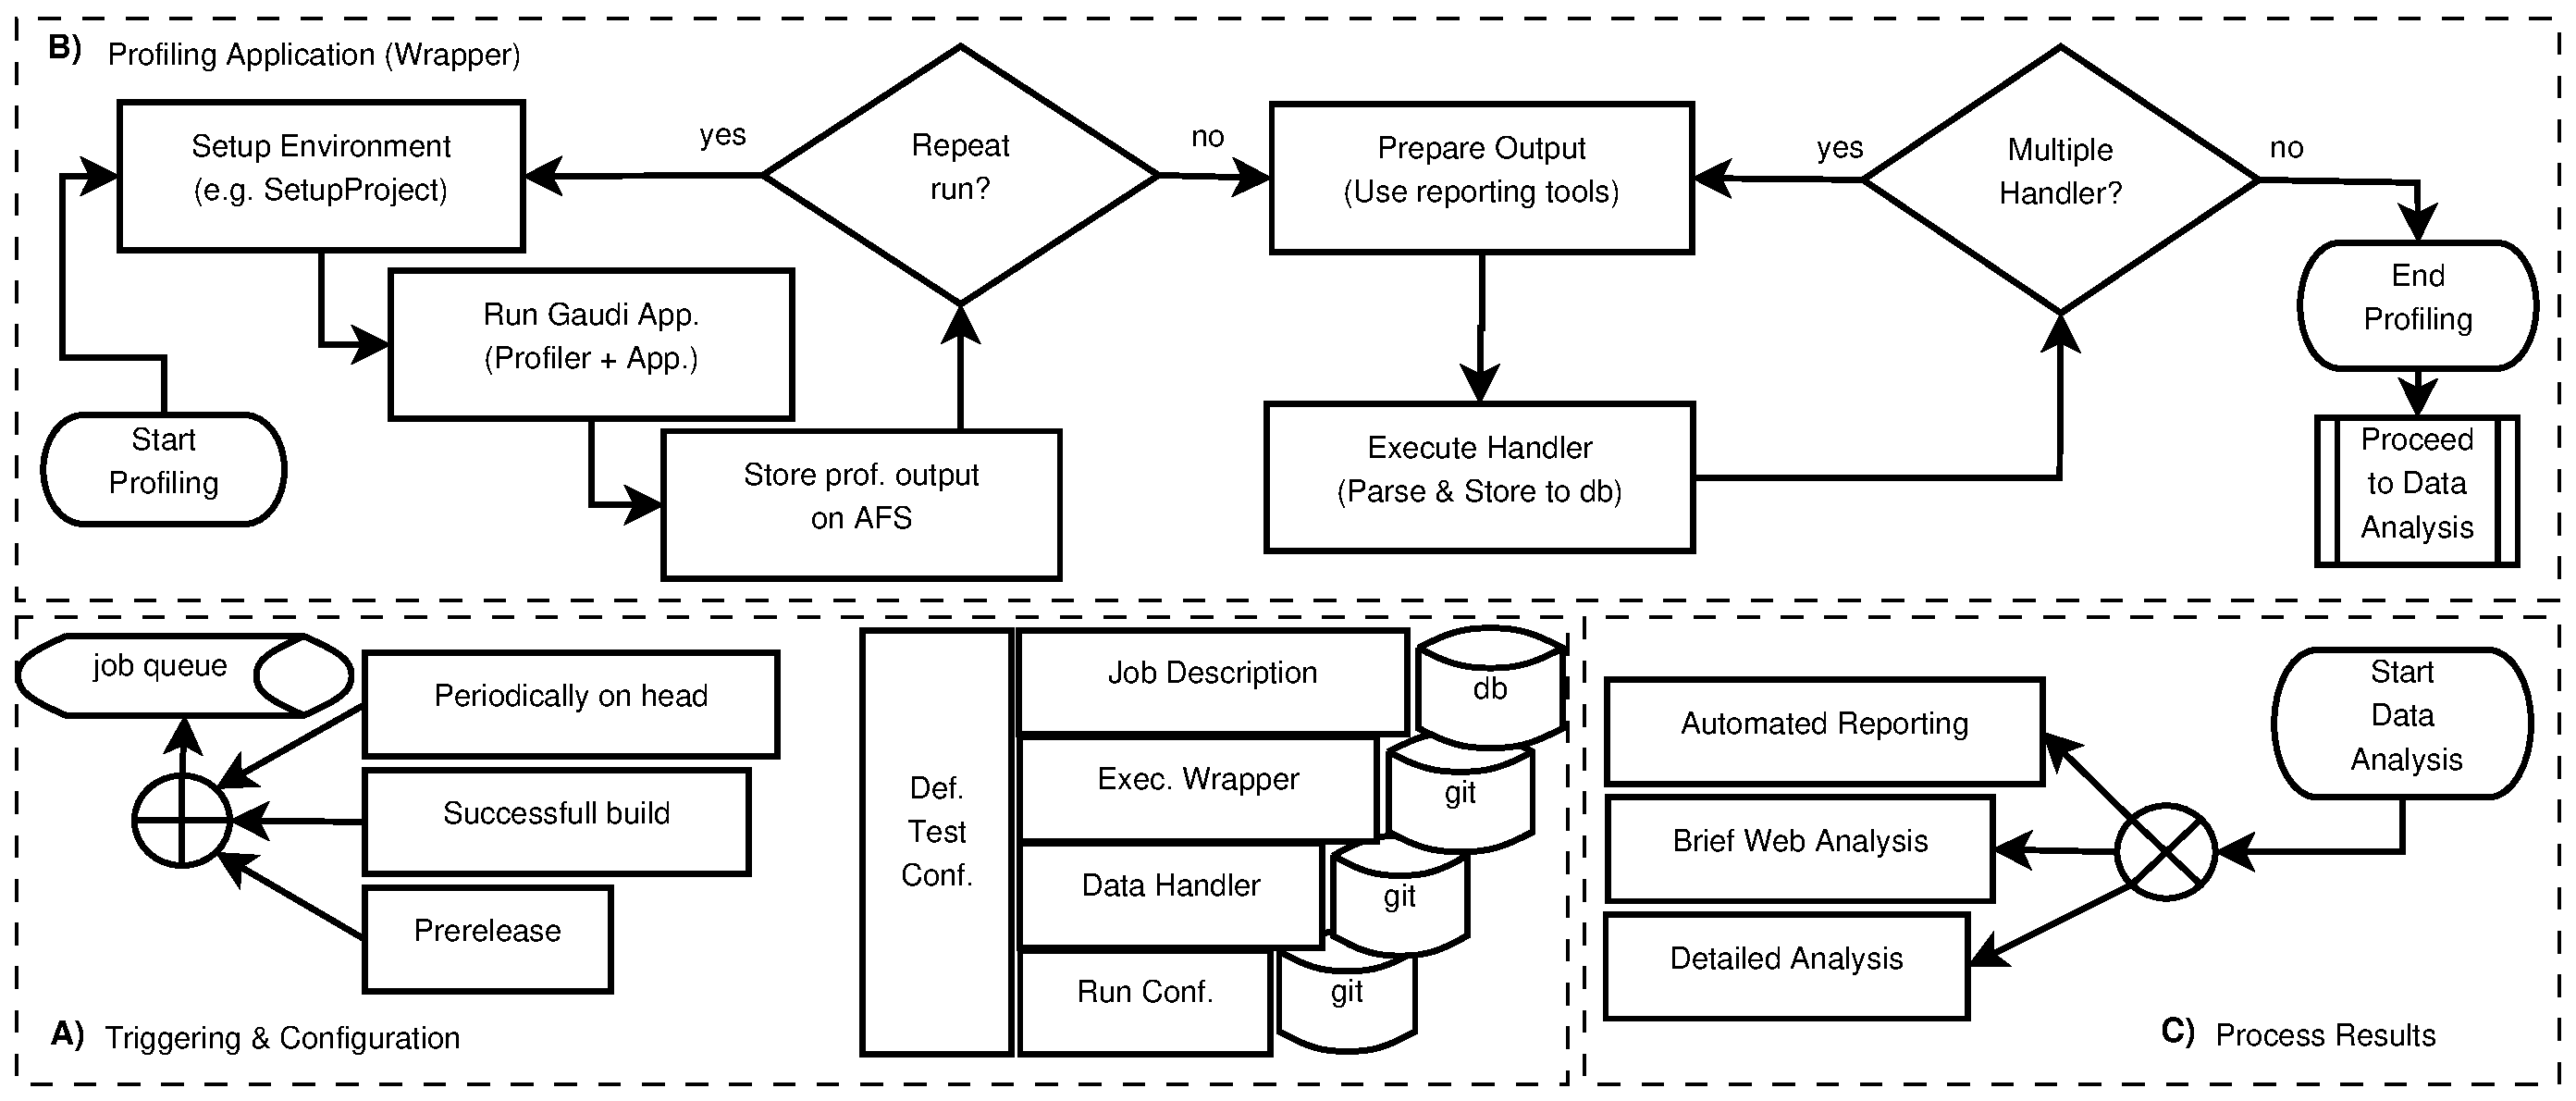
\includegraphics[scale=0.3]{figures/profiling_process.eps}
\caption{\small \textit{nix}}
\label{fig:trend}
\end{figure}

\section{The LHCb PR framework}
\label{sec:lhcbpr_framework}

The LHCb PR platform uses the continous integration system Jenkins \cite{jenkins} to prepare, configure and schedule jobs for profiling, a set of wrappers to customize available profilers for their working environment, a set of data handlers to parse and collect output data from the profilers, a SQL database to store summarized data and the web analysis framework LHCb PR. 

\subsection{Structure}
\label{sec:structure}

\begin{itemize}
 \item Job distribution and triggering
 \item Job execution and profiling
 \item Data collection
 \item Web-based Analysis platform
 \item Test definition
\end{itemize}

\subsection{Job distribution and triggering}
\label{sec:job_distribution}

To facilitate regular and intensive systematic profiling, Jenkins is used to manage the job distribution to the test platform. This makes the in- or exclusion of other platforms simple and avoids interference between multiple runs on the same machine. The configuration (creation) of Jobs can further be used for a test specific pre-installation and compilation for development specific purposes or to run pre-configured jobs before new releases are tagged.
\newline
An other advantage is that the job configuration in Jenkins can be used for regular execution to call a validation test of recent builds from the build system to perform a subsequent profiling procedure.  

\subsection{Execution and Profiling}
\label{sec:execution_and_profiling}

Commercial and open-source profilers becoming more and more available. The open source community developed crucial tools like the valgrind tool suit. Other tools like google's tcmalloc can be used to elaborate processing time and memory consumption. Additional, recent hardware features give access to hardware counters of the PMU (performance monitoring unit), which can be read from proprietary software like intels VTune or open source projects like oprofile.
\newline
This paper is not going to evaluate the benefits and drawbacks of different tools, but wants to enable a profiling platform like LHCb PR to individually setup these tools on their specific necessary way. For these purposes scripts are collected into a separate repository which can easily execute the test cases and stay flexible for individual configuration. To improve the configuration of profiling runs and to focus the profiling onto main time consuming parts, integration of the profilers instrumentation methods are highly recommended.

\subsection{Data collection}
\label{sec:data_collection}

Data collection can be done in three different ways, first one can segregate information from the results of profilers, store files containing performance information and store the resting profiler specific collected information. Segregating information can also be quite diverse depending on which profiler were delivering the information. To maintain flexibility here, a collection of data handler were written for each profiler in use. They have to parse the output, select and combine information and finally collect it for insertion into the LHCb PR underlying database.  

\subsection{Test cases}
\label{sec:test_cases}

Use cases are importend 

\subsubsection{Use case Reconstruction}
\label{sec:use_case_rec}

\subsubsection{Use case High-Level-Trigger}
\label{sec:use_case_hlt}

\begin{figure}[t]
\begin{minipage}[t]{17pc}
\includegraphics[scale=0.4]{figures/trend_brunel.png}
\caption{\small \textit{nix}}
\label{fig:trend}
\end{minipage}\hspace{1pc}%
\begin{minipage}[t]{17pc}
\includegraphics[scale=0.4]{figures/overview_brunel.png}
\caption{\small \textit{nix}}
\label{fig:overview}
\end{minipage}
\end{figure}

\section{Performance analysis}
\label{sec:performance_analysis}

The core of the LHCb performance and regression (PR) framework is its customized analysis platform based on Django \cite{django}.

\subsection{Web based analysis}
\label{sec:web_based_analysis}

\subsection{Detailed analysis}
\label{sec:detailed_analysis}

\section{Conclusions}
\label{sec:conclusions}

Using a customizable platform to collect and summarize profiling results enables the LHCb collaboration to focus on important places in Gaudi algorithms during the refactoring time and beyond. This is organized in a way that takes additional tasks away from developers and simplifies the profiling to introduce a certain level of automation, e.g. for performance validation before a new release. It permits an arbitrary level of flexibility due to including new profilers and to monitor new software performance and quality values. The web front-end simplifies the task of monitoring the general performance of the Gaudi frameworks applications. 

\section*{References}
\begin{thebibliography}{3}
\bibitem{gaudi} G. Corti, M. Cattaneo, P. Charpentier, F. Markus, P. Koppenburg, P. Mato, F. Ranjard, S. Roiser, I. Belyaev and G. Barrand, ``Software for the LHCb experiment'', IEEE Transactions on Nuclear Science, vol. 53, nb. 3, P.1323-1328, 2006
\bibitem{intel_auditor} A. Mazurov and B. Couturier, ``Advanced Modular Software Performance Monitoring'', J. Phys.: Conf. Ser. 396 052054, 2012
\bibitem{monitoring} D. F. Kruse and K. Kruzelecki, ``Modular Software Performance Monitoring'', J. Phys.: Conf. Ser. 331 042014, 2011
\bibitem{django} ``Django is a high-level Python Web framework'', url: https://www.djangoproject.com/
\bibitem{jenkins} ``Jenkins, An extendable open source continuous integration server'', url: https://www.jenkins-ci.org/
\end{thebibliography}
\end{document}
